\subsection{IoT Stream Processing Applications}
\begin{alltt}TODO\scriptsize 0.75/1 pages
\end{alltt}
As part of the application tutorial we have picked a specific class of streaming applications, i.e. IoT applications that are concerned with interpreting and conceptualizing sensor data in real-time. Here we describe applications in two distinct domains. The first domain relates to Sports and Entertainment in which quantifiable insights about sports and entertainment events are created from sensors deployed at a venue. The second domain relates to Industry 4.0 in which sensor data from production machines is used to reduce energy costs and operations and maintenance costs. The application examples are based on commercial deployments that run on top of AGT International's \footnote{\url{http://www.agtinternational.com}} Internet of Things Analytics (IoTA) platform. 

We use the two domains for two purposes: (1) With the applications described for sports and entertainment we illustrate the specific characteristics of IoT streaming applications and the associated challenge of choosing an appropriate streaming infrastructure. (2) We use the applications for Industry 4.0 to illustrate how stream processing applications can be benchmarked using the HOBBIT benchmarking platform.

\subsubsection{Sports and Entertainment}
Applications we consider in the sports and entertainment domain provide real-time narratives about key events that are happening at such an event. This way it is not necessary to watch the whole event, but one can be notified in real-time about highlights at the event based on insights created form the sensor data. A concrete example of such events are basketball matches in which various sensors provide the necessary data. For instance smart shirts worn by players, microphones deployed to monitor the audience, and cameras and wristbands are sensors that have been successfully used in commercial deployments. Data from these sensors in combination with play-by-play data can be used to recognize behaviour, emotions, activities, actions, pressure and other physical aspects about a game. These insights are related to players, teams, fans and family and are preferably provided as semantic data streams. Semantic data access decouples applications from data providers and enables domain experts to better work with the data, e.g. for generating content and distributing it via social media. The application and the underlying technical architecture has been recently described at AWS re:invent\footnote{\url{https://www.portal.reinvent.awsevents.com/connect/sessionDetail.ww?SESSION_ID=14367}}.
%Figure Basketball ?

Other applications in this domain include mixed martial art fights, professional bull riding and the detection of event highlights at mass sport events such as the Color Run. For mixed martial arts many sensors including cameras, smart floors and a sensor embedded in a fighter's glove\footnote{\url{http://mmajunkie.com/2017/12/ufc-219-artificial-intelligence-glove-sensors-approved-by-nsac}} can be used based on which a range of insights including punch strength and fighter's stress level are derived. Here it is important that insights can be delivered in real-time without noticeable delay compared to a broadcast of the fight. The full application scenario has been described in a recent keynote at AWS re:invent\footnote{\url{https://youtu.be/vataVq9gY_o}}.

\begin{center}
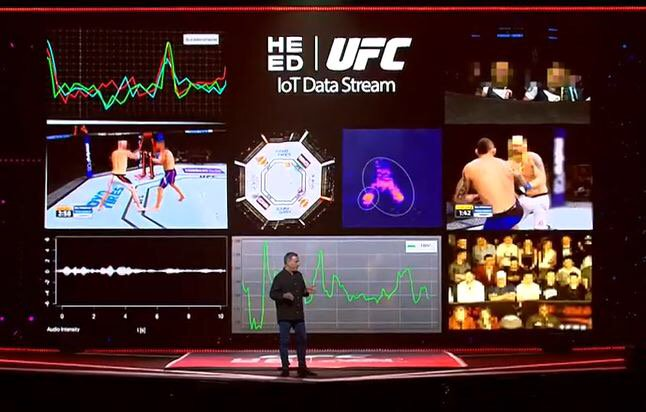
\includegraphics[scale=0.3]{pictures/DP6L8S9XkAYFMCw.jpg}
\captionof{figure}{A sample of IoT data streams that can be obtained during a fight.}
\end{center}

In professional bull riding, sensors that are attached to riders and bulls have been successfully used in order to quantify the bull's and rider's performance\footnote{\url{https://www.businesswire.com/news/home/20170822006048/en/Heed-Accelerates-Growth-Ground-Breaking-Partnerships-Professional-Basketball}}. As this information is among others used for automatic scoring, it is of particular importance that analytic results are available as soon as the ride is finished. 

In a similar fashion we use a range of wearable sensors for creating event highlights for participants at mass sport events. In the CPaas.io project \footnote{\url{http://www.cpaas.io}} we have developed an application that uses action cameras and fitness bands to automatically detect event highlights based on runner's activity, emotions, dance energy levels, and many more metrics. In this application real-time aspects include scenarios in which event highlights are being directly sent to friends of the participants. 

\subsubsection{Industry 4.0}
In the area of Industry 4.0 we considered two applications. The first application is related to the challenge of reducing energy costs while the second challenge is related to reducing maintenance cost. Electricty bills of industrial consumers contain a pricing component that incurs higher charges for higher peaks of electrical load. For a small to medium enterprise avoiding such peak load events can lead to significant savings \cite{strohbach_and_toll_2016}. This can be achieved by predicting expected peaks e.g. up to 30 minutes ahead of time and taking counter measures such as temporarily switching off high energy consumers such as air conditioning. 

The second application focuses on detection of anomalous machine states in order to reduce maintenance costs. For instance, in injection molding machines a sudden high energy consumption may indicate that an injection nozzle is jammed and checking the machine may avoid further damage. This applicaiton is described in more detail in section \ref{subsubsec:benchmarking}.

\subsubsection{Choosing the Streaming Infrastructure}
When choosing a streaming infrastructure fulfilling the requirements of the above application scenarios, we face the following challenges

\begin{itemize}
  \item Lack of standardized query language for streaming applications 
  \item Flexibility for Programming Languages
  \item Low Latencies and short-lived stream processing pipelines
% semantic mapping has been briefly mentioned in the sports and entertainment app
%  \item Semantic mapping
\end{itemize}

While in the database world there are standardized query languages such as SQL and SPARQL, there is still no standard stream processing language (see Section \ref{sec:tut_lang}). As a consequence streaming applications are very closely coupled to the underlying stream processing system making the choice of the infrastructure a critical one. 

When considering the applications above, it becomes apparent that the implementation of a variety of analytical modules are required. However, there is a discrepancy between the tools and programming languages typically used by data scientist (Python, Julia, C/C++, R, Matlab, etc.) and the mainly JVM based languages (Java and Scala) that are supported in common stream systems as described in section \ref{sec:tut_systems}. Although python is increasingly supported in these systems, resource management of JVM external languages is badly supported. However, such external resources may be considerable, e.g. if machine learning models are involved. And languages other than Python are not directly supported at all.

Finally, IoT streaming applications as described above require low latency processing pipelines rather than supporting an extremely high number of throughput. In addition there may be a large number of short-lived rather than a few long-lived processing pipelines. In typical settings there may thousands of sensor streams connected to the system and a multitude of analytical results created from all the streams. However, not all streams are equally important at all times. For instance, in a sports tournament there may be a couple of standard pipelines being set up for the duration of the tournament, but many more smaller pipelines are set up for the duration of a single match, half or quarter. Some pipelines are only set up, based on ad-hoc queries. For the shorter-lived pipelines it is extremely important that the pipeline including its analytics module can be set up extremely fast, i.e. below one second, including tasks such as the deployment and resource allocation of analytics module and the models they use. To our knowledge virtually all existing and mature frameworks focus on high throughput and long lived processing pipelines and thus do not fully support these requirements. 

\subsubsection{Benchmarking IoT Streaming Applications}\label{subsubsec:benchmarking}

In order to objectively measure some of these requirements we have co-organized the DEBS Grand Challenge 2017 \cite{gulisano_et_al_2017}. In particular we were interested in low latencies and processing RDF data. As applications we asked participants to detect anomalies in injection molding machines. The original data set has been provided by Weidmüller\footnote{\url{http://www.weidmueller.de}} and used to create a mimicked data set that closely resembles the original data set. This has been necessary as the original data cannot be provided for confidentiality reasons. As an additional benefit this approach allows the generation of data sets of virtually any size. The data set is available from the HOBBIT Data Set Portal\footnote{\url{https://hobbit.iminds.be/dataset/weidmuller}}.

Systems under test had to correctly answer a pre-defined query that describes an anomaly in the expected machine states. The task involved to find k cluster centers in a sliding window in order to identify the machine states. As a next step, it was required to build a Markov model over the sliding window and use it to determine the probability of the last N state transitions. Finally, if the probability is below a given threshold the system under test had to report an anomaly. Machines could dynamically leave and join.

The systems under test were benchmarked with the HOBBIT benchmarking platform \footnote{\url{https://project-hobbit.eu/outcomes/hobbit-platform}} that ensured that we could objectively quantify the performance of a distributed stream processing pipeline. As we used a pre-defined algorithm for detecting anomalies, we expected full correctness from all systems and compared latency and also measured throughput. Overall 14 teams participated in the challenge,  and 7 past the correctness test. The fastest system \cite{amariei_et_al_2017} achieved an average latency of about 39ms. The DEBS Grand Challenge 2017 benchmark is openly available as part of the HOBBIT platform. 
